

%%% BEGIN CHAPTER 3 SINGLECELL %%%

%% Paper title page %%
\chapter[Single--cell analysis defines the divergence between the \\ innate lymphoid cell lineage and lymphoid tissue--inducer cell lineage]{Single--cell analysis defines the divergence between the innate lymphoid cell lineage and lymphoid tissue--inducer cell lineage}

% authors
Isabel E Ishizuka\U{1,2,6}, Sylvestre Chea\U{3,6}, Herman Gudjonson\U{1,4-6}, Michael G Constantinides\U{1,2}, Aaron R Dinner\U{4,5}, Albert Bendelac\U{1,2,7} and Rachel Golub\U{3,7}
\\ \\
\U{1}Committee on Immunology, University of Chicago, Chicago, Illinois, USA. 
\U{2}Department of Pathology, University of Chicago, Chicago, Illinois, USA. 
\U{3}Institut Pasteur, Immunology Department, Lymphopoiesis Unit, Inserm U668, University Paris Diderot, Paris, France. 
\U{4}Institute of Biophysical Dynamics, University of Chicago, Chicago, Illinois, USA. 
\U{5}Department of Chemistry, University of Chicago, Chicago, Illinois, USA. 
\U{6}These authors contributed equally to this work. 
\U{7}These authors jointly directed this work. 
\\
Correspondence should be addressed to A.B. (abendela@bsd.uchicago.edu).
\\ \\
Author contributions: I.E.I., H.G., M.G.C. and A.B. designed the experiments; I.E.I. performed single-cell sorting and culture experiments; S.C. designed and performed the lymphoid Biomark assay; H.G. performed computational analysis of the Biomark experiments; M.G.C. designed and performed experiments; A.R.D. supervised computational analysis; A.B. supervised experiments; R.G. supervised Biomark experiments; and I.E.I., H.G. and A.B. wrote the manuscript with contributions from all authors.
\\ \\
Published in Nature Immunology January 18, 2016; doi:10.1038/ni.3344

\newpage
\section{ABSTRACT}

The precise lineage relationship between innate lymphoid cells (ILCs) and lymphoid tissue–inducer (LTi) cells is poorly understood. Using single-cell multiplex transcriptional analysis of 100 lymphoid genes and single-cell cultures of fetal liver precursor cells, we identified the common proximal precursor to these lineages and found that its bifurcation was marked by differential induction of the transcription factors PLZF and TCF1. Acquisition of individual effector programs specific to the ILC subsets ILC1, ILC2 and ILC3 was initiated later, at the common ILC precursor stage, by transient expression of mixed ILC1, ILC2 and ILC3 transcriptional patterns, whereas, in contrast, the development of LTi cells did not go through multilineage priming. Our findings provide insight into the divergent mechanisms of the differentiation of the ILC lineage and LTi cell lineage and establish a high-resolution 'blueprint' of their development.

\section{INTRODUCTION}

Innate lymphocytes lack B cell or T cell antigen receptors and exert effector functions at mucosal barriers \cite{diefenbach2014,serafini2015}. These populations segregate into three general groups on the basis of their expression of the transcription factors T-bet, GATA-3 and \RORgt. However, there is considerable heterogeneity among T-bet-expressing group 1 lymphocytes, which comprise conventional (or classical) natural killer (NK) cells (cNK cells), group 1 innate lymphoid cells (ILC1 cells) and tissue-resident NK cells, and among \RORgt-expressing group 3 lymphocytes, which comprise CCR6\UP lymphoid tissue-inducer (LTi) cells and CCR6\UM ILC3 cells. In addition, some plasticity has been reported among CCR6\UM ILC3 cells, which can upregulate T-bet expression and acquire group 1 properties \cite{klose2013}, and among some populations of ILC2 cells, which can acquire group 3 properties \cite{huang2015}.

Lineage-tracing and cell-transfer studies have suggested that ILC1, ILC2 and ILC3 cells, but not LTi cells or cNK cells, are derived from a common dedicated precursor, the ILC precursor (ILCP), characterized by expression of the transcription factor PLZF \cite{constantinides2014}. Similar to the LTi precursor (LTiP), the ILCP originates from a lymphoid precursor that expresses the integrin \ab{} and is itself derived from the common lymphoid precursor (CLP). The Id2\U{hi} fraction of \ab\UP lymphoid precursors, called 'common helper innate lymphoid precursors' (CHILPs), is a heterogeneous population that includes the PLZF-expressing ILCPs as well as precursors of LTi cells \cite{klose2014}, but whether the CHILP population includes a common precursor of both ILCs and LTi cells or separate precursors of each lineage has not yet been determined. A study has suggested that cNK cells might originate from an earlier Id2\U{lo}CXCR6\UP fraction of \ab-expressing lymphoid precursors (\aLPs) \cite{yu2014}. Thus, the developmental relationships between these lineages remain incompletely established.

Several transcription factors, including Nfil3, Tox, Id2, GATA-3, TCF-1 (encoded by \textit{Tcf7}) and PLZF (encoded by \textit{Zbtb16}) \cite{constantinides2014,yu2014,xu2015,seillet2014,seehus2015, hoyler2012,serafini2014,yagi2014,yang2013,mielke2013,moro2010}, are required for the development of all or several of these innate lineages, which suggests they have an effect at a common precursor stage. However, partial defects, rather than complete defects, have often been reported in mice lacking these transcription factors, which suggests substantial redundancy and complexity of this early transcriptional network. Other transcription factors have been found to selectively affect individual ILC lineages, such as the effect of \RORa{} (encoded by \textit{Rora}), Bcl-11b and Gfi1 in ILC2 cells \cite{wong2012,spooner2013,walker2015}, which suggests more distal effects in the ILC-differentiation pathway. Precise understanding of the general hierarchy of expression of these factors is missing, however, which limits the design and interpretation of mechanistic studies aiming at delineating their interplay.

Here we used cultures of single cells purified from the fetal livers of a mouse reporter strain expressing green fluorescent protein (GFP) and Cre recombinase from the gene encoding PLZF (\textit{Zbtb16}-GFP-Cre) to precisely define the differentiation stages between CLP and ILC and to identify the stage of divergence between ILCs and LTi cells. We also performed multiplex quantitative single-cell transcriptional analysis of 100 lymphoid genes to characterize the complexity of molecular events associated with this differentiation pathway. We derived a high-resolution map and inferred a precise ordering of the induction of transcription factor expression and identified previously unknown stages of development before and after PLZF expression and the stage of bifurcation between the ILC lineage and LTi cell lineage. Notably, transcriptional priming for the different cytokine effector programs occurred at the ILCP stage itself through multilineage priming. In contrast, the LTiP proceeded to directly acquire its type 3 program without undergoing mixed transcriptional priming. Together our findings further define the dichotomy between ILCs and LTi cells and provide new insight into the stages and mechanisms of their development and the interplay of transcription factors that direct their differentiation.

\section{RESULTS}

\subsection{Bifurcation of \aLPs into ILCPs and LTiPs}
Lin\UM IL-7R$\alpha$\UP fetal liver cells (where lineage (Lin) is defined by a 'cocktail' of antibodies to \CDte, TCR$\beta$, CD19, CD11c, GR-1, Ter119 and NK1.1) included CLPs, identified by a Flt3\UP \ab\UM{} profile, and a cell population expressing \ab, which included the precursors to innate lymphoid lineage, thought to arise from the CLP (Fig. \ref{fig:chap3_F1}a). This \ab-expressing population was originally called '\aLP', but the identification of ILCPs and LTiPs among \aLPs prompted us to limit the designation of '\aLP' to the \ab-expressing cells that were neither ILCP nor LTiP but include their precursors \cite{serafini2015,moro2015}. We further subcategorized this \aLP population as an Flt3\UP subset and Flt3\UM subset to identify early precursors and late precursors, respectively. We detected these populations by flow cytometry among fetal liver cells obtained from the \textit{Zbtb16}-GFP-Cre reporter strain at embryonic day 15 (E15) (Fig. \ref{fig:chap3_F1}a). Among the Lin\UM IL-7R$\alpha$\UP \ab\UP{} population, the ILCPs were identified by GFP expression, and the LTiPs were identified by their GFP\UM CXCR5\UP profile \cite{constantinides2014,cherrier2012}. The LTiPs were clearly distinguishable from the other subsets in this staining, although a small fraction of these cells seemed to have low expression of GFP (Fig. \ref{fig:chap3_F1}a). As expected, only the LTiPs coexpressed the chemokine CCR6 and the coreceptor CD4 (Fig. \ref{fig:chap3_F1}b).

%% Chapter 3 Figure 1 aLP subpopulations %%
\begin{figure}[h]
\begin{center}
	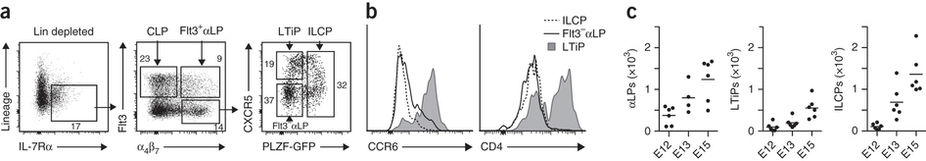
\includegraphics[width=\textwidth]{figures/chapter3/F1}
\end{center}
	\caption{Identification of distinct subpopulations of \ab-expressing lymphoid precursors in fetal liver.} 
	(a) Flow cytometry of fetal liver cells from E15 Z \textit{Zbtb16}-GFP-Cre reporter mice after depletion of Lin\UP cells (expressing \CDte, CD11c, CD19, NK1.1, TCR$\beta$, Ter119 and GR-1) by magnetic bead–based cell separation and staining for IL-7R$\alpha$ (left), Flt3 and \ab{} (middle) and CXCR5 (right), for the identification of distinct subpopulations representing CLPs, \aLPs, LTiPs and ILCPs (middle and right) after gating on Lin\UM IL-7R$\alpha$\UP{} cells (left). Numbers adjacent to outlined areas indicate percent cells in each subpopulation. (b) Flow cytometry of ILCPs, LTiPs and Flt3\UM{} \aLPs stained for CCR6 or CD4. (c) Quantification of \aLPs, LTiPs and ILCPs in fetal liver at E12, E13 and E15. Each symbol represents an individual fetus; small horizontal lines indicate the mean. Data are representative of twelve independent experiments (a) or three experiments (b) or are pooled from two independent experiments (c).
	\label{fig:chap3_F1}
\end{figure}

Both LTiPs and ILCPs could already be detected at a low frequency among Lin\UM IL-7R$\alpha$\UP \ab\UP{} fetal liver cells at E12, the earliest time point of our analysis, and their absolute numbers increased five- to tenfold by E15 (Fig. \ref{fig:chap3_F1}c). To establish the lineage relationships among \aLPs, ILCPs and LTiPs, we performed single-cell cultures of \aLP subsets (Flt3\UP and Flt3\UM) on OP9 stromal cells in the presence of interleukin 7 (IL-7) and stem-cell factor, as described5. We categorized the growing cells as ILC1 colonies, ILC2 colonies or ILC3 colonies by high expression of the activating NK cell receptor NK1.1, the costimulatory receptor ICOS or \ab, respectively, as reported5. We distinguished LTi cells from ILC3 colonies by expression of CD4, which was expressed by nearly half the LTi cells but not by ILC3 cells (Fig. \ref{fig:chap3_F1}b), although this method underestimated the real frequency of LTi cell colonies by approximately twofold. We were unable to distinguish cNK cells from ILC1 cells by expression of eomesodermin (Eomes), because expression of this transcription factor was induced in ILC1 cells in our culture conditions (data not shown). However, because fetal progenitor cells do not produce cNK cells \cite{constantinides2015}, we counted all NK1.1\UP colonies as ILC1 cells.

ILCPs gave rise nearly exclusively to single and mixed colonies of ILC1 cells, ILC2 cells and ILC3 cells (Fig. \ref{fig:chap3_F2}), consistent with this cell type's being a common precursor to these lineages, as reported \cite{constantinides2014}. In contrast, Flt3\UP{} and Flt3\UM{} \aLPs also generated a sizeable proportion of LTi cells, which indicated that this group of cells included precursors to the LTi cell lineage. Notably, many wells containing LTi cells also included ILC1 cells or ILC2 cells (the presence of ILC3 cells could not be ascertained in wells containing LTi cells), which indicated that a single Flt3\UP{} or Flt3\UM{} \aLP precursor could generate both LTi cells and ILC lineages. Thus, while the reported CHILP population \cite{klose2014} included a heterogeneous mixture of ILCPs and other precursors, our observations identified the Flt3\UM{} \aLP as the common proximal precursor, at the single-cell level, of both ILCPs and LTiPs.

%% Chapter 3 Figure 2 aLP potential %%
\begin{figure}[p]
\begin{center}
	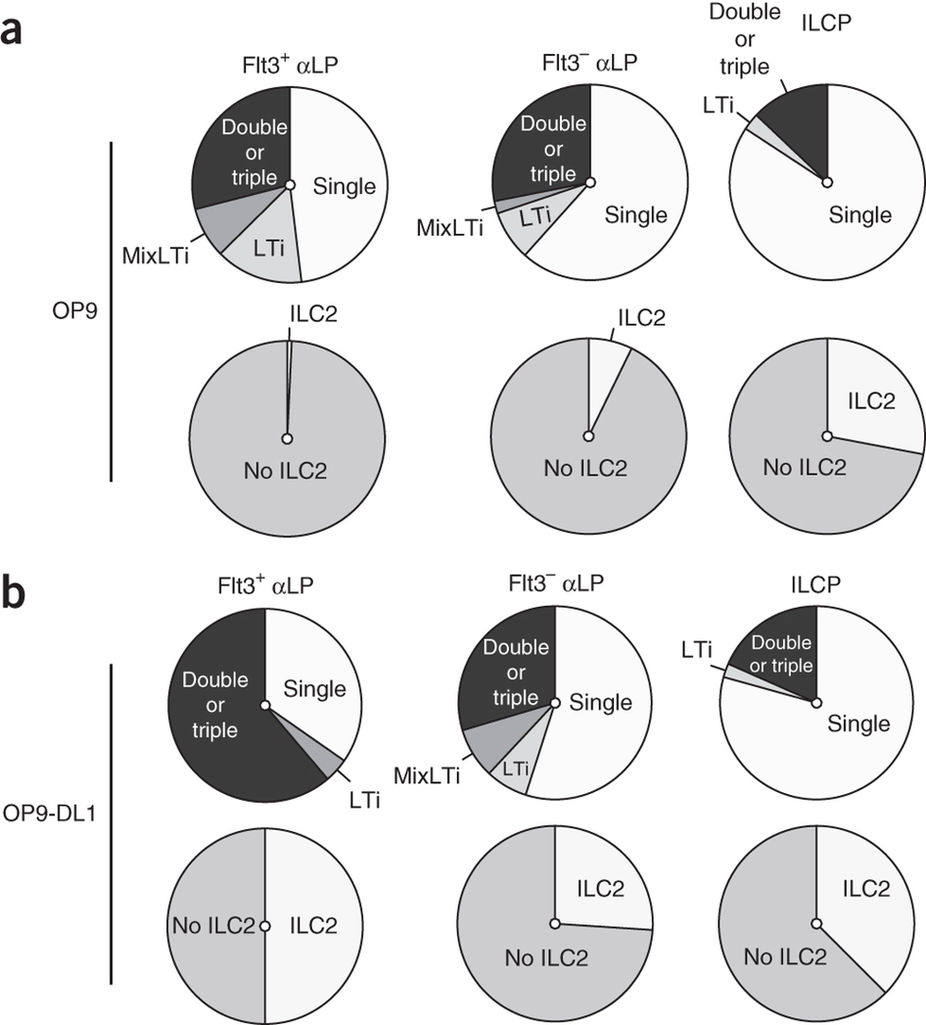
\includegraphics[height=0.5\textheight]{figures/chapter3/F2}
\end{center}
	\caption{Colonies derived from single-cell cultures of \ab-expressing lymphoid precursors in fetal liver.} 
	Frequency of single ILC1, ILC2 or ILC3 cells (Single) or two or more ILC subsets (Double or triple), LTi cells, and mixed colonies of LTi (CD4\UP) cells plus either ILC1 cells or ILC2 cells (the presence of ILC3 cells could not be ascertained in these wells) (MixLTi) (top), and frequency of wells containing ILC2 colonies (whether single or mixed with other ILC lineages) (bottom), among single-cell cultures of various precursors sorted from \textit{Zbtb16}-GFP-Cre fetal livers at E14–E16 and cultured with OP9 cells (a) or OP9-DL1 cells (b). Average cloning efficiency, 31-64\%; $<$3\% of colonies could not be characterized by staining and are not presented here. In OP9-DL1 cultures, colonies of pro-T cells were also observed in 47\% of Flt3\UP \aLP wells, 19.7\% of Flt3\UM{} \aLP wells and 14.5\% of ILCP wells; these were identified by a CD4\UP or CD8\UP, ICOS\UM \ab\UM NK1.1\UM phenotype (data not shown). Data are pooled from at least three independent experiments (OP9) or one to three independent experiments (OP9-DL1) with 51-447 total colonies for each progenitor population.
	\label{fig:chap3_F2}
\end{figure}

Notably, when we performed the cultures with OP9 stromal cells lacking the DL1 ligand of Notch receptors, we found that many fewer ILC2 colonies were derived from Flt3\UP{} \aLPs or Flt3\UM{} \aLPs than from ILCPs (Fig. \ref{fig:chap3_F2}a, bottom). However, this defect was largely corrected in OP9-DL1 cultures (Fig. \ref{fig:chap3_F2}b, bottom). This finding was consistent with the proposal that a Notch signal is essential for ILC2 differentiation \cite{yang2013,wong2012} and further established that the signal must be delivered early at the \aLP stage, rather than late at the ILCP stage. Together these experiments demonstrated that the fetal liver \aLP pathway was dedicated to the formation of the ILC and LTi cell lineages. They also identified the late Flt3\UM \aLP as the common proximal precursor to ILCPs and LTiPs.

\subsection{Single-cell multiplex quantitative RT-PCR of ILC precursors}

We used multiplex quantitative RT-PCR for transcriptional analysis of single cells along the fetal pathway linking \aLPs to ILCPs and LTiPs, with a panel of 100 probes for genes encoding lymphoid development factors, including transcription factors, cytokine receptors and chemokine receptors. Data from 339 single cells, including 157 \aLPs, 168 ILCPs and 14 LTiPs, were compiled from two independent single-cell sorting experiments with pooled E15 fetal livers. After filtering results by the expression of 'housekeeping' (control) genes, we considered the transcriptional profiles from 299 single cells for downstream analysis.

Unsupervised hierarchical clustering analysis of these transcriptional profiles defined groups of cells that seemed to be in distinct developmental stages (Fig. \ref{fig:chap3_F3}). Consistent with the proposal that acquisition of PLZF expression signified a distinctive developmental transition for ILCs, we found strong, visually evident separation of the transcriptional profiles of the \aLP populations (Fig. \ref{fig:chap3_F3}, left) and ILCP populations (Fig. \ref{fig:chap3_F3}, right). We used contiguous branches of the hierarchical clustering dendrogram to define three clusters of predominantly \aLPs (AI-AIII), one cluster composed of mixed \aLPs and ILCPs (B), and four clusters of predominantly ILCPs (CI-CIV), on the basis our understanding of ILC development. All clusters were distinct from one another and were composed of a substantial number ($>$20) of similar cells (Supplementary Fig. \ref{fig:chap3_S1}). One additional cluster of about 20 cells, all with conspicuously high expression of \textit{Il1rl1} (which encodes the IL-33 receptor chain IL-33R$\alpha$), was removed from the study because it was unrelated to the other clusters and instead seemed to represent contaminating mast cell precursors with low expression of \ab and PLZF (Supplementary Fig. \ref{fig:chap3_S2}). Thus, this analysis identified further heterogeneity among precursor cells and generated a 'blueprint' of their temporal sequence during ILC development.

%% Chapter 3 Figure 3 hierarchical clustering %%
\begin{figure}[h]
\begin{center}
	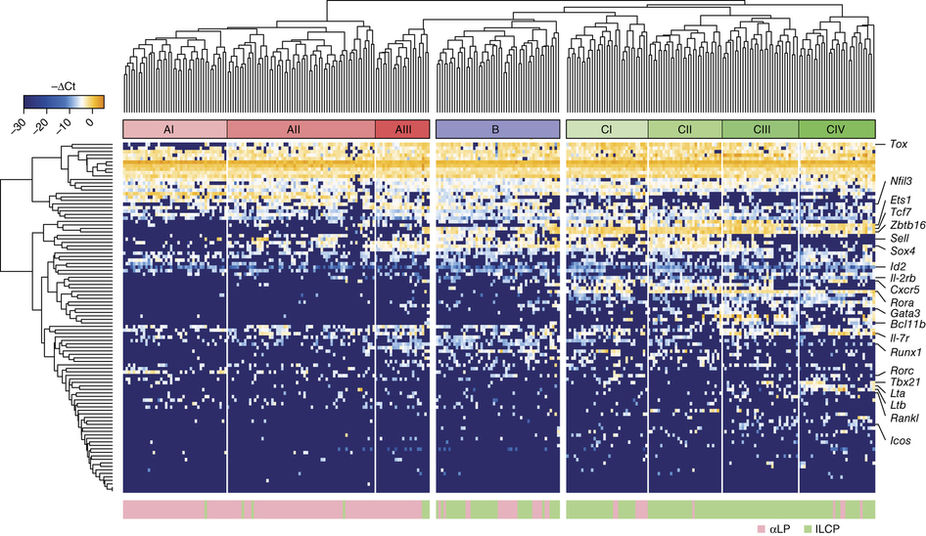
\includegraphics[width=\textwidth]{figures/chapter3/F3}
\end{center}
	\caption{Hierarchical clustering distinguishes \aLP and ILCP transcriptional profiles.} 
	Hierarchical clustering dendrogram (top and left margin) derived from single-cell multiplex quantitative PCR analysis of 299 single \aLPs and ILCPs, distinguishing clusters AI–-AIII (\aLPs; left), cluster B (mixed \aLPs and ILCPs; middle), and clusters CI–-CIV (ILCPs; right); each column represents a single cell (bottom, sorted cell type; key, bottom right), and each row represents one gene (of 100 total; right margin, select genes encoding products with known or anticipated roles in ILC development). $\Delta$Ct (top left key), difference in threshold cycle relative to the average value for the 'housekeeping' (control) gene. Data are from two independent experiments with 157 \aLPs and 168 ILCPs from pooled livers.
	\label{fig:chap3_F3}
\end{figure}

\subsection{Early developmental transitions}

To facilitate analysis of the clusters identified above, we generated a condensed heat map of gene expression in all 299 single cells, limited to a set of 20 key informative genes. Consistent with \aLPs' being early precursors to ILCPs and LTiPs, there was sparse expression of genes encoding transcription factors and cytokines specific for these lineages in the A clusters. For example, \textit{Zbtb16}, \textit{Tcf7}, \textit{Gata3}, \textit{Bcl11b}, \textit{Cxcr5}, \textit{Rorc}, \textit{Rora} and \textit{Tbx21} were not expressed by clusters AI-AIII (Fig. \ref{fig:chap3_F4}). In contrast, clusters AI-AIII expressed genes encoding transcription factors linked to early ILC and LTi development, including \textit{Id2}, \textit{Tox}, \textit{Nfil3}, \textit{Sox4}, \textit{Ets1} and \textit{Runx1} (Fig. 4a). That conclusion was confirmed by plotting of the average mRNA expression per cell (Fig. \ref{fig:chap3_F4}b) and the frequency of cells expressing genes encoding these transcription factors in each cluster (Supplementary Fig. \ref{fig:chap3_S3}). Notably, a distinct temporal pattern of expression could be inferred from these plots. Thus, cells in cluster AI had low expression of \textit{Id2}, but most lacked expression of \textit{Tox} and \textit{Nfil3} (Fig. \ref{fig:chap3_F4}). Nearly all cells in clusters AII and AIII, however, expressed \textit{Tox} and \textit{Nfil3} (Fig. \ref{fig:chap3_F4}). Cells in clusters AI and AII lacked expression of \textit{Ets1}, \textit{Sox4} and \textit{Runx1}, whereas a majority of cells in cluster AIII expressed these genes (Fig. \ref{fig:chap3_F4}). Finally, \textit{Tcf7} and \textit{Zbtb16} were not expressed by clusters AI-AIII (\aLPs) but were widely expressed in cluster B and the C clusters (ILCPs) (Fig. \ref{fig:chap3_F4}). We measured low Id2 expression across clusters AI-AIII and found a tendency toward more frequent and higher expression in cluster B and clusters CI-CIV (Fig. \ref{fig:chap3_F4}), in line with the suggestion that increased \textit{Id2} expression is correlated with commitment to innate lineages \cite{klose2014}. Thus, our analysis suggested that the temporal patterns of expression of these transcription factors were precisely regulated. Furthermore, unlike \textit{Tox}, whose expression remained high, \textit{Nfil3} was ultimately downregulated in ILCP clusters (Fig. \ref{fig:chap3_F4}b), consistent with its temporally limited requirement, as suggested by experiments of late gene ablation \cite{xu2015}.

%% Chapter 3 Figure 4 early transitions %%
\begin{figure}[h]
\begin{center}
	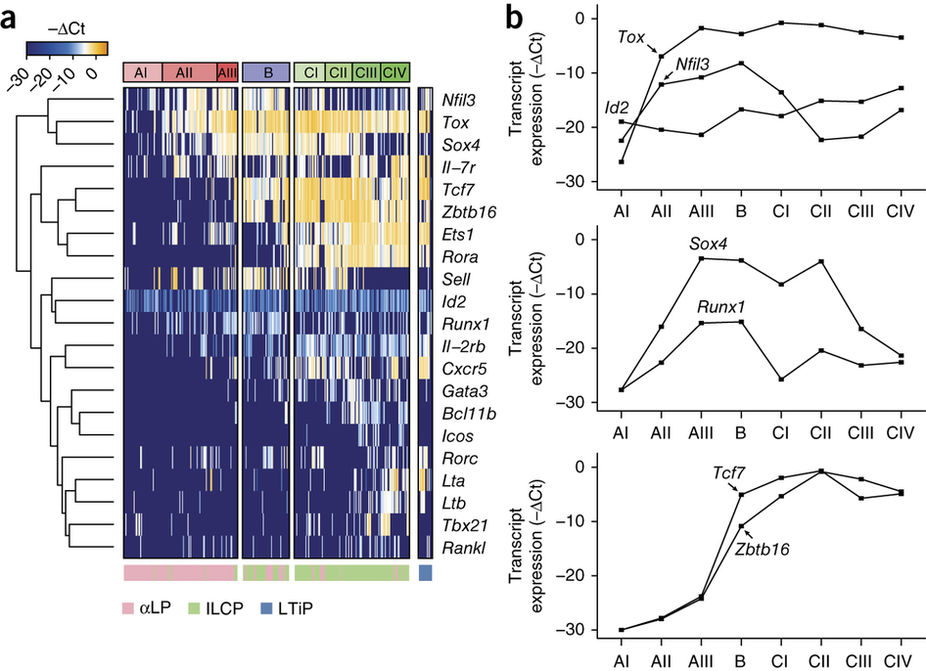
\includegraphics[width=\textwidth]{figures/chapter3/F4}
\end{center}
	\caption{Clusters define the developmental progression of key transcription factors.} 
	(a) Single-cell multiplex quantitative PCR (as in Fig. 3) of transcripts from genes encoding products with known or anticipated roles in ILC development, ordered by hierarchical clustering of \aLPs and ILCPs as in (Fig. \ref{fig:chap3_F3}), and of LTiPs (far right); below, sorted cell type (key, bottom left). (b) Transcript expression (average $\Delta$Ct values) for genes encoding products that define early developmental transitions in each cluster.
	\label{fig:chap3_F4}
\end{figure}

\subsection{Bifurcation of ILC and LTi cell branches}

Cluster B comprised the most mixed representation of \aLPs and ILCPs and seemed to be a developmental transition state linking early developmental events and specification to the ILC lineage versus the LTi cell lineage. Notably, cells in cluster B expressed \textit{Tcf7} and \textit{Zbtb16} but largely lacked expression of genes encoding ILC lineage–specific factors (Fig. \ref{fig:chap3_F4}). In fact, the expression of \textit{Tcf7} and \textit{Zbtb16} was lower in cluster B than that in ILCP clusters (Fig. \ref{fig:chap3_F4}), which confirmed the conclusion that cluster B corresponded to a transitional stage. A similar pattern was found for \textit{Id2} (Fig. \ref{fig:chap3_F4}), suggestive of developmental continuity between \aLP clusters and ILCP clusters, with cluster B probably including the first cells to acquire \textit{Zbtb16} expression before specification to the ILC lineage. Although the induction of \textit{Tcf7} and \textit{Zbtb16} seemed to be nearly synchronous, a fraction of cluster B cells expressed \textit{Tcf7} without \textit{Zbtb16} (Fig. \ref{fig:chap3_F4} and Supplementary Fig. \ref{fig:chap3_S3}), which suggested that this fraction might have included cells destined to the LTi cell lineage. In fact, detailed analysis of cells in cluster B that expressed \textit{Tcf7} but not \textit{Zbtb16} showed that most of these cells had a tendency to express genes encoding factors associated with the LTi cell lineage, including \textit{Rorc}, while conspicuously lacking expression of \textit{Rora}, which is expressed in more mature LTiPs (Fig. \ref{fig:chap3_F5}). In contrast, cells in cluster B that expressed both \textit{Tcf7} and \textit{Zbtb16} rarely expressed \textit{Rorc} at that stage and instead displayed some expression of genes encoding factors associated with ILC lineages, such as \textit{Gata3}, while they lacked \textit{Rora} expression (Fig. \ref{fig:chap3_F5}); this suggested that they were less mature than most ILCPs. Thus, we concluded that cluster B represented the stage of bifurcation of the \aLP into the LTi cell and ILC lineages.

%% Chapter 3 Figure 5 ILC LTi branching %%
\begin{figure}[h]
\begin{center}
	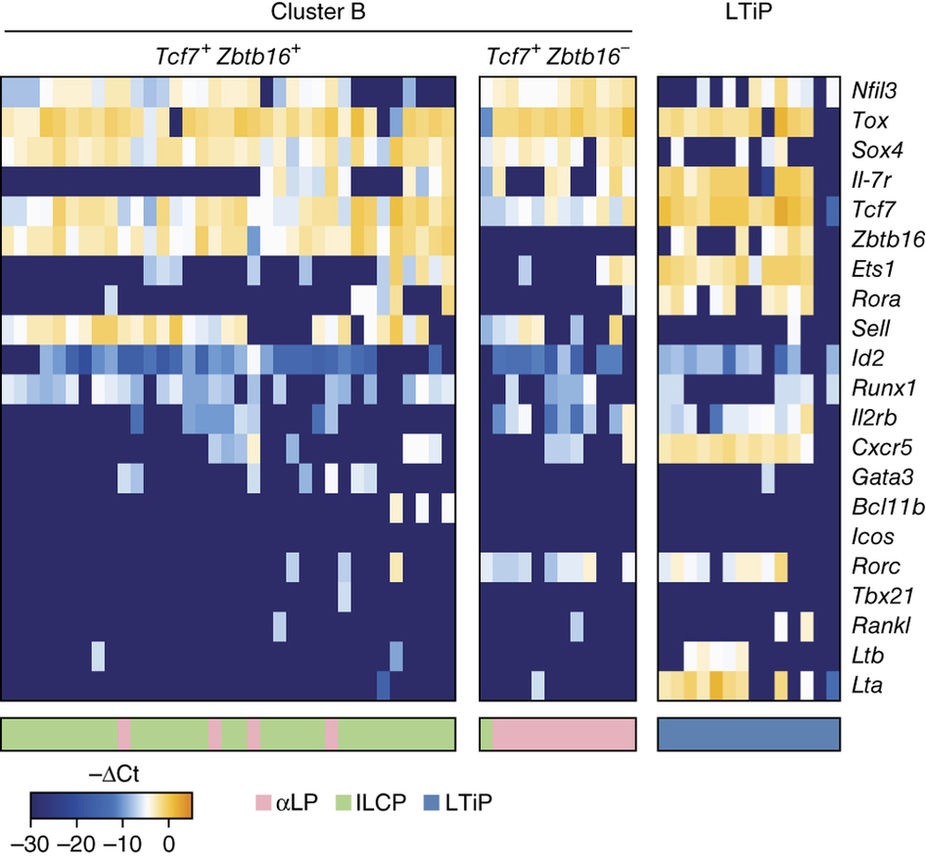
\includegraphics[width=0.5\textwidth]{figures/chapter3/F5}
\end{center}
	\caption{Transitional cluster B includes two distinct subsets, on the basis of expression of \textit{Tcf7} and \textit{Zbtb16}.} 
	Transcript expression by cells from cluster B that express both \textit{Tcf7} and \textit{Zbtb16} (\textit{Tcf7}\UP \textit{Zbtb16}\UP) or express \textit{Tcf7} but not \textit{Zbtb16} (\textit{Tcf7}\UP \textit{Zbtb16}\UM) (Fig. \ref{fig:chap3_F3}), and of LTiPs (right).
	\label{fig:chap3_F5}
\end{figure}

\subsection{ILC lineage differentiation originates in the ILCP}

Cells in the ILCP clusters (CI-CIV) showed signs of ILC maturation and expressed genes encoding ILC lineage-defining transcription factors and cytokines (Fig. \ref{fig:chap3_F4}). These cells had almost universally high expression of \textit{Zbtb16}, \textit{Tcf7} and \textit{Id2}, and additional transcripts further distinguished them from the developmentally intermediate cluster B. Almost all cells in ILCP clusters expressed \textit{Ets1} and \textit{Rora} and tended to have low \textit{Nfil3} expression. The ILCP clusters delineated by hierarchical clustering probably reflected sequential stages of ILC maturation, rather than association with particular ILC lineages. Cells in clusters CI and CII had high expression of \textit{Sell} and \textit{Sox4} that diminished in clusters CIII and CIV. Conversely, cells in clusters CIII and CIV had higher expression of Ets1 and Il7r than that of cells in clusters CI and CII. Characteristically, cells in clusters CIII and CIV more frequently expressed genes encoding ILC lineage-defining transcription factors, including \textit{Tbx21}, \textit{Bcl11b} and \textit{Rorc}, than did cells in clusters CI and CII. Our finding of the expression of genes encoding ILC lineage-defining transcription factors in multiple ILCP clusters indicated that we were probably capturing developmental stages of ILC differentiation. Furthermore, cells that expressed genes encoding ILC lineage-defining transcription factors in later clusters (clusters CIII and CIV) tended to express genes encoding other lineage-associated cytokines and transcription factors and thus seemed to be more differentiated.

\subsection{ILCPs undergo multilineage transcriptional priming}

To better assess the range of cells among the ILCP clusters that seemed to be differentiating toward ILC lineages, we compiled a subset of cells that expressed genes encoding ILC lineage-associated factors (Fig. \ref{fig:chap3_F6}). Specifically, we identified cells with ILC1, ILC2 or ILC3 markers by their expression of \textit{Tbx21} (ILC1) or \textit{Bcl11b} (ILC2) or at least two genes among \textit{Cxcr5}, \textit{Rorc}, \textit{Lta} and \textit{Ltb} (ILC3). In this population, we observed many cells coexpressing genes encoding markers of different ILC lineages, such as \textit{Tbx21} and \textit{Bcl11b}, or \textit{Tbx21} and \textit{Cxcr5}, or \textit{Tbx21} and \textit{Rorc}, and even cells expressing multiple markers of the three different lineages. In total, among 120 total cells in ILCP clusters, we found 60 cells that expressed genes encoding lineage-differentiation markers, of which nearly one third (19) coexpressed genes encoding markers of different lineages.

%% Chapter 3 Figure 6 ILC multilineage %%
\begin{figure}[h]
\begin{center}
	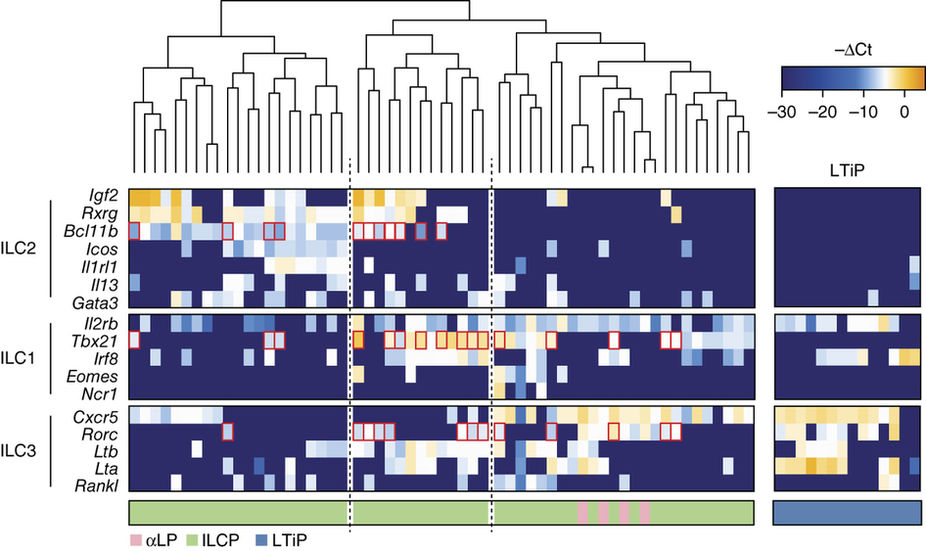
\includegraphics[width=0.7\textwidth]{figures/chapter3/F6}
\end{center}
	\caption{Multilineage transcriptional priming in ILCPs.} 
	Expression of ILC lineage-specific transcripts (left margin) in differentiating ILCPs and in LTiPs (far right); red outlines indicate single cells expressing multiple genes encoding lineage-specific transcription factors (two or more genes among \textit{Bcl11b}, \textit{Tbx21} or \textit{Rorc}). Below, sorted cell type (key, bottom left).
	\label{fig:chap3_F6}
\end{figure}

The multilineage priming noted above was substantiated by the expression of genes encoding additional lineage-specific factors (Fig. \ref{fig:chap3_F6}). In particular, the simultaneous expression of \textit{Bcl11b} and \textit{Icos} was associated with expression of canonical ILC2 genes, including \textit{Il1rl1} and \textit{Il13}. We also observed increased expression of \textit{Gata3} in \textit{Bcl11b}-expressing cells, although \textit{Gata3} was expressed throughout ILCPs without strict lineage association (as shown before by flow cytometry \cite{constantinides2014}). Across cells in ILCP clusters, we observed a relatively strong correlation between the expression of \textit{Rxrg} and \textit{Igf2} and that of \textit{Bcl11b}. The expression of \textit{Tbx21} was associated with higher expression of \textit{Il2rb} and, in some cases, with expression of \textit{Eomes} and \textit{Ncr1} (which encodes the activating receptor NKp46). We also found that \textit{Irf8} expression seemed to be associated with \textit{Tbx21} expression in differentiating ILCPs. Finally, we found that expression of \textit{Rorc} was associated with high expression of \textit{Cxcr5}, as well as with expression of \textit{Lta}, \textit{Ltb} and \textit{Rankl}. Generally, expression of \textit{Il2rb} and \textit{Cxcr5} was observed throughout the ILCP clusters, with higher expression and greater frequency of expression associated with the expression of genes encoding other ILC1 and ILC3 factors. There was substantial overlap between the expression of genes encoding ILC1 and ILC3 factors, in particular for the expression of \textit{Tbx21} and \textit{Cxcr5}, \textit{Lta}, \textit{Ltb} and \textit{Rankl}.

The results noted above were in contrast to the expression profile of LTiPs in the same fetal livers (Figs. \ref{fig:chap3_F5} and \ref{fig:chap3_F6}). These cells showed no evidence of multilineage priming. In particular, they conspicuously lacked expression of \textit{Gata3}, \textit{Bcl11b} or \textit{Tbx21}, which further supported the proposal that they follow a distinct lineage-differentiation pathway.

Collectively, the expression of genes encoding multiple lineage factors in ILCP clusters was suggestive of multilineage potential. This further confirmed the proposal that cells navigating ILC lineage 'decisions' were in the ILCP population. Moreover, it suggested that during the initial lineage 'decisions', the relationships among distinct ILC lineage factors are more complicated than might have been anticipated from studies of helper T cells, for example.

\subsection{Transcriptional programs correlate with lineage 'decisions'}

To functionally evaluate the relevance of the transcriptional programs noted above in ILCPs, we assessed their lineage potential in single-cell cultures. We sorted fetal ILCP subsets on the basis of their expression of the cytokine receptor chain CD122 (IL-2R$\beta$), ICOS and the chemokine receptor CXCR5 (Fig. \ref{fig:chap3_F7}a) and studied their progeny in single-cell cultures. We found that these subsets showed some bias toward the corresponding ILC1 or ILC2 program (Fig. \ref{fig:chap3_F7}b, top). Thus, the earliest precursors with a bias toward the ILC1 lineage or ILC2 lineage could be discerned at the ILCP stage by their CD122\UP CXCR5\UM{} profile or ICOS\U{hi} profile, respectively (Fig. \ref{fig:chap3_F7}a). However, the biases were incomplete, indicative of the residual multipotency of these populations. For example, while ICOS\U{hi} ILCPs generated mostly ILC2 colonies, they also gave rise to some single ILC1 and ILC3 colonies, as well as to dual and triple colonies (Fig. \ref{fig:chap3_F7}b). In contrast, CD122\UP CXCR5\UM{} ILCPs generated mainly ILC1 colonies but also generated some single ILC3 colonies as well as dual colonies (Fig. \ref{fig:chap3_F7}b). Even the ILCPs that produced dual colonies maintained a corresponding bias as, for example, all dual colonies originating from ICOS\U{hi} precursors included an ILC2 colony, and those originating from a CD122\UP CXCR5\UM{} precursor included an ILC1 colony (Fig. \ref{fig:chap3_F7}b, bottom). Together with the multilineage priming observed at the transcriptional level, these observations indicated that lineage polarization was proceeding by stepwise restriction of alternative programs from multipotential precursors, which ultimately led to the canonical polarized lineages. Using intracellular staining of transcription factors, we further confirmed that a substantial fraction of fetal ILCPs coexpressed T-bet, \RORgt{} and GATA-3 or ICOS, indicative of multilineage priming, whereas mature ILCs were strictly limited to expression of their lineage-specific transcription factors (Fig. \ref{fig:chap3_F7}c). This scenario is different from current models of the polarization of helper T cells, wherein acquisition of cytokine effector programs does not typically involve intermediates with mixed lineage patterns.

%% Chapter 3 Figure 7 flow multilineage %%
\begin{figure}[p]
\begin{center}
	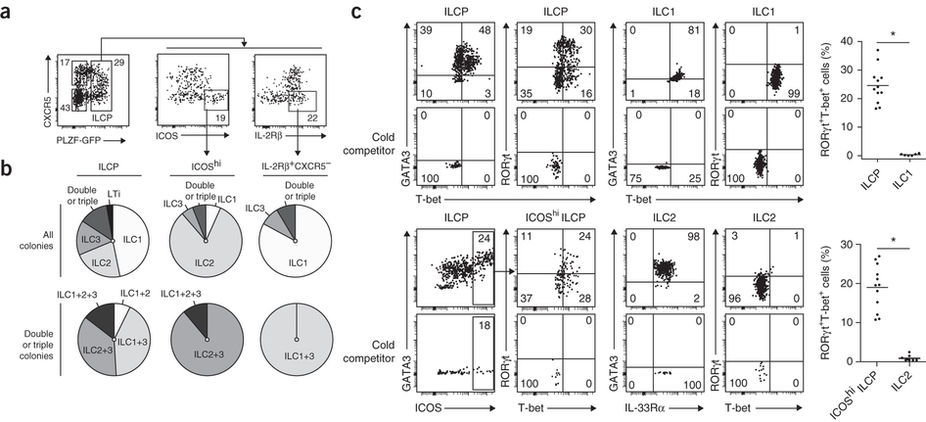
\includegraphics[width=0.9\textwidth]{figures/chapter3/F7}
\end{center}
	\caption{ILCP subsets with biased progeny in single-cell cultures.} 
	(a) Flow cytometry of fetal liver ILCPs, identified by GFP (PLZF) expression (as in Fig. \ref{fig:chap3_F1}) and sorted on the basis of expression of CXCR5, ICOS and IL-2R$\beta$. Numbers adjacent to outlined areas indicate percent cells in each subpopulation. (b) Distribution of single colonies and double or triple colonies (top) and the composition of double or triple colonies (bottom) from each progenitor cell. ILCP, n = 425 colonies; IL-2R$\beta$\UP CXCR5\UM{} ILCP, n = 82 colonies; ICOS\U{hi} ILCP, n = 150 colonies. (c) Intracellular staining of various transcription factors in fetal ILCPs at E14 (n = 12; gated as Lin\UM IL-7R$\alpha$\UP \ab\UP PLZF\UP) and in ILC1 cells from mature adult liver (n = 6; gated as \CDte\UM NK1.1\UP CD49a\UP) or ILC2 cells from adult bone marrow (n = 7; gated as Lin\UM IL-7R$\alpha$\UP Thy1\UP Sca1\UP), in the presence of unlabeled antibody (cold competitor) added before the conjugated antibody used for staining (bottom row of each group) or in the absence of such unlabeled antibody (top row of each group). Numbers adjacent to outlined areas or in quadrants indicate percent cells in each. Each symbol (far right) represents an individual mouse; small horizontal lines indicate the mean. *$P < 0.0001$ (two-tailed Student's t-test). Data representative of at least three experiments (a), are pooled from one to six independent experiments (b) or are representative of two independent experiments (c).
	\label{fig:chap3_F7}
\end{figure}

\section{DISCUSSION}

Using the \textit{Zbtb16}-GFP-Cre reporter system, we have identified the stage at which the \aLP bifurcates into ILCPs or LTiPs during early fetal lymphopoiesis. We also used single-cell multiplex quantitative PCR analysis to produce a high-resolution map of the development of innate lymphocyte lineages. We emphasize that the proposed developmental progression discussed below is inferred on the basis of the continuity of gene expression between clusters but remains to be experimentally demonstrated.

We found that \textit{Zbtb16} and \textit{Tcf7} were simultaneously upregulated in cluster B at the bifurcation of the ILC and LTi cell lineages, with \textit{Tcf7} expression marking both lineages and \textit{Zbtb16} expression identifying the ILC lineage. A fraction of the precursor cells that expressed \textit{Tcf7} but did not express \textit{Zbtb16} expressed \textit{Rorc} and seemed closer to LTiPs than to ILCPs. Notably, cells in cluster B lacked expression of \textit{Rora}, which is characteristically induced later in development, in further support of the conclusion that cells in cluster B navigate the bifurcation between the LTi cell lineage and ILC lineage.

The A clusters before the induction of \textit{Zbtb16} and \textit{Tcf7} must therefore represent earlier precursor cells, on the basis of the expression of \textit{Id2}, \textit{Tox}, \textit{Nfil3} and \textit{Runx1} (refs. \cite{yu2014,xu2015,seillet2014, seehus2015,moro2010,tachibana2011,aliahmad2010,yokota1999}), which has been linked to both lineages. \textit{Id2} seemed to be the earliest expressed transcription factor–encoding gene with substantial expression in cluster AI, a stage at which \textit{Nfil3} and \textit{Tox} transcripts were barely detected. Expression of \textit{Nfil3} and \textit{Tox} rapidly ascended during the transition to cluster AII and reached maximal levels in cluster AIII. These findings stand in apparent contrast to a published report showing that Nfil3 can bind to and induce Id2 and that ablation of Nfil3 can be complemented by Id2 (ref. \cite{xu2015}) but are consistent with the presence of \textit{Id2} transcripts reported in arrested precursor cells lacking expression of \textit{Nfil3} or \textit{Tox} \cite{xu2015,seehus2015}. Nfil3 might therefore exert a positive feedback loop rather than being a primary trigger for \textit{Id2} expression. The expression of Nfil3 and that of Tox also seemed to be induced nearly simultaneously. Thus, a report that Nfil3 can induce \textit{Tox} and that ablation of \textit{Nfil3} can be complemented by Tox7 might also reflect a positive feedback mechanism.

Additional transcription factor–encoding genes that were induced early after \textit{Id2}, \textit{Tox} and \textit{Nfil3} but before \textit{Zbtb16} and \textit{Tcf7} included \textit{Sox4}, \textit{Runx1} and \textit{Ets1}. Although the function of the transcription factors encoded is currently unknown, Sox4 has been associated with the development of fetal \gdT cells in conjunction with TCF-1 (ref. \cite{malhotra2013}), whereas Runx1 has been shown to be important for the development of NK cells and LTi cells \cite{tachibana2011}, and Ets1 has been associated with NK cell development \cite{ramirez2012}. Thus, these factors are probably integral components of the early transcriptional network of innate lymphocytes.

Clusters CI-CIV defined several stages of ILCPs, with cluster CI associated with the induction of \textit{Rora}, which was maintained in all ILC lineages, although it seems to be required only for ILC2 cells \cite{wong2012,halim2012}. Cluster CII was associated with \textit{Gata3} expression, which was maintained at a high level during the remaining ILCP stages and ultimately is downregulated in mature ILC1 and ILC3 cells \cite{constantinides2014}. Therefore, transient but high \textit{Gata3} expression is an intrinsic developmental event that might distinguish ILC3 cells from LTi cells. Clusters CIII and CIV were marked by emergence of the expression of genes encoding lineage-specific factors. Notably, there was a distinct and extensive pattern of coexpression of genes encoding factors from the three different lineages in nearly a third of these cells, which indicated that a phase of multilineage transcriptional priming preceded the polarization of mature lineages. In contrast, the LTiPs did not go through this singular process and directly expressed Rorc and other genes encoding attributes of the LTi cell lineage without coexpression of genes encoding alternative ILC lineage markers. The extent of multilineage priming revealed by our study goes beyond the coexpression of low levels of T-bet and \RORgt{} by GATA3\UP{} ILC precursors detected in the fetal intestine by flow cytometry \cite{bando2015}. Indeed, we found that multilineage priming included an extended list of genes encoding canonical markers of all three lineages. ILCPs sorted on the basis of the expression of genes encoding some of these lineage differentiation markers showed a relative bias in differentiation toward the corresponding lineages after single-cell culture, although these subsets also maintained some multipotency, as shown by the generation of mixed colonies. These findings suggested that the terminal differentiation of ILCPs into polarized ILC lineages is more complex than previously envisaged. Instead of directly acquiring one of three programs, precursors of ILCs first activated multiple effector programs simultaneously and then progressively turned off priming of alternative lineages. In the absence of exogenous polarizing cytokines, such a developmental strategy can take advantage of the well-established antagonistic effects between these programs \cite{zhu2010}. In ILCPs, external or internal inputs that might influence lineage 'decisions' include retinoids, which have been shown to favor type 3 innate lymphocytes \cite{van2014,spencer2014}, or Notch signals, which are needed for ILC2 cells \cite{yang2013,neill2010}. Multilineage transcriptional priming has been proposed as a more general strategy for developmental 'decisions', such as the differentiation of various hematopoietic lineages from a common progenitor \cite{laslo2006,hu1997,miyamoto2002,Ng2009}. It has not been widely reported for programs used in the differentiation of CD4\UP{} helper T cells into the TH1, TH2 or TH17 subset of helper T cells, which instead rely on polarizing cytokines released during infection or allergy \cite{zhu2010}, although mixed transcriptional patterns have been observed in cells cultured under mixed cytokine conditions \cite{antebi2013}.

Our studies further emphasize that although they share many functional properties, ILC3 cells and LTi cells have distinct precursors and different developmental histories. Only precursors of ILC3 cells transited through a stage of high expression of \textit{Zbtb16} and \textit{Gata3} with multilineage priming at the single-cell level. Our results should encourage studies aimed at further elucidation of the different functions of LTi cells and ILC3 cells, as illustrated, for example, by a report that ILC3 cells and LTi cells have different topographical locations in the lamina propria \cite{satoh2014}.

In summary, our study has allowed the identification of several previously unknown developmental transitions and transcription factors sequentially associated with the lineage progression of innate lymphocytes. In particular, our results characterized in cellular and molecular detail the previously poorly defined bifurcation of lymphoid precursors into LTiPs and ILCPs. They have also demonstrated differential mechanisms of the acquisition of polarized effector programs by these lineages.


\section{METHODS}

\textit{Mice.}
\textit{Zbtb16}-GFP-Cre reporter mice were generated in our laboratory as described and contain an internal ribosome entry site after the final exon of \textit{Zbtb16}, followed by a fusion gene encoding enhanced GFP–Cre recombinase\cite{constantinides2014}. For fetal ontogeny experiments, the morning a vaginal plug was identified was counted as embryonic day 0 (E0). Mice were housed in a specific pathogen–free environment at the University of Chicago and experiments were performed in accordance with the guidelines of the Institutional Animal Care and Use Committee.
\\
\textit{Preparation of cell suspensions.}
Fetal livers were mechanically dissociated through a 70-$\mu$m cell strainer and resuspended in HBSS (Gibco) containing 0.25\% BSA (Sigma-Aldrich) and 5 mM sodium azide (Sigma-Aldrich).
\\
\textit{Flow cytometry.}
Cell suspensions were pre-incubated with BD Fc Block for 10 min on ice. Fetal liver cells were pre-enriched for \ab-expressing cells unless otherwise indicated. For pre-enrichment of \ab\UP cells, fetal liver or bone marrow cells were stained with allophycocyanin (APC)-conjugated antibody and were subsequently bound to anti-APC microbeads (Miltenyi Biotec). The cells were then enriched using the autoMACS (Miltenyi Biotec) positive-selection double-sensitive program. Lineage (\CDte, CD11c, CD19, NK1.1, TCR$\beta$, Ter119 and GR-1) depletion of fetal liver or bone marrow cells was accomplished by incubation of cells with biotinylated antibodies to lineage markers antibodies (identified below) and then binding to streptavidin-conjugated microbeads (Miltenyi Biotec) and separation using the autoMACS depletion-sensitive program. Fluorochrome- or biotin-conjugated monoclonal antibodies to the following were used (clone number in parentheses): to mouse \ab (DATK32), CCR6 (29-2L17), CD11c (N418), CD19 (6D5), CD27 (LG.3A10), CD90.2 (Thy-1.2; 53-2.1), CD122 (5H4), CD127 (IL-7R$\alpha$; A7R34), CXCR5 (L138D7), Fc$\epsilon$RI$\alpha$ (MAR-1), GR-1 (RB6-8C5), ICOS (C398.4A), IL-33Rα (ST2; DIH9), NKp46 (29A1.4), Sca-1 (D7), Ter119 (TER-119), T-bet (4B10), mouse IgG1 $\kappa$-chain (MG1-45), mouse IgG2a $\kappa$-chain (MG2a-53) and rat IgG2b $\kappa$-chain (RTK45-30) (all from BioLegend); \CDte (145-2C11), CD4 (GK1.5), CD8$\alpha$ (53-6.7), CD45.1 (A20), CD45.2 (104), CD49a (Ha31/8), NK1.1 (PIK136), TCR$\beta$ (H57-597) and \RORgt (Q31-378) (all from BD Biosciences); and GATA3 (TWAJ; eBioscience). The D-9 antibody to PLZF was conjugated to Alexa Fluor 647 using the labeling kit from Molecular Probes Life Technologies. For intracellular staining, cells were fixed and permeabilized using the Foxp3 Transcription Factor Staining Buffer Set (eBioscience). Cells were then blocked with unlabeled isotype-matched control antibody (identified above). As negative control, a 20-fold excess of unlabeled antibody to the transcription factor was added before the conjugated antibody ('cold' competition). Data were acquired on a LSRII (BD Biosciences) or cells were sorted using a FACSAria II (BD Biosciences) and data were analyzed using FlowJo software (TreeStar).
\\
\textit{Single-cell cultures.}
Stocks of OP9 and OP9-DL1 stromal cells were a gift from J.C. Zúñiga-Pflücker. All experiments were performed in Opti-MEM with GlutaMAX (Gibco) containing 10\% FCS (Gibco), 1\% penicillin-streptomycin (Gibco), and 60 mM 2-mercaptoethanol (Sigma-Aldrich) and were maintained in a 37 °C incubator (Thermo Scientific) with 5\% CO2. Stromal cells were plated at 70\% confluency. Before addition of lymphocytes, stromal cells were irradiated (1,500 rads) and culture media supplemented with murine IL-7 (25 ng/ml; BioLegend) and stem-cell factor (25 ng/ml; BioLegend). Fetal liver lymphocyte samples underwent enrichment for \ab\UP{} cells by MACS and were sorted as single cells onto 96-well plates containing stromal cells and cytokines as described above. Cultures were analyzed after 6 or 10 d of culture and only colonies with more than ten CD45.2\UP{} cells were considered.
\\
\textit{Biomark.}
Cells were sorted in 96-well quantitative PCR plates in 10 μl of a CellsDirect One-Step quantitative RT-PCR Kit (Life Technologies), containing mixtures of diluted primers (0.05x final concentration). Preamplified cDNA was obtained after reverse transcription (15 min at 40 °C, 15 min at 50 °C and 15 min at 60 °C), and preamplification (22 cycles: 15 s at 95 °C and 4 min at 60 °C), and diluted 1: 5 in TE pH8 Buffer (Ambion). Sample mix was as follows: diluted cDNA (2.9 $\mu$l), Sample Loading Reagent (0.29 $\mu$l; Fluidigm), TaqmanUniversal PCR Master Mix (3.3 $\mu$l; Applied Biosystem) or Solaris quantitative PCR Low ROX Master Mix (3.3 $\mu$l; GE Dharmacon). The assay mix was as follows: Assay Loading Reagent (2.5 $\mu$l; Fluidigm), Taqman (2.5 $\mu$l; Applied Biosystem) or Solaris (2.5 $\mu$l; GE Dharmacon). A 48.48 or 96.96 dynamic array integrated fluidic circuit (IFC; Fluidigm) was primed with control line fluid, and the chip was loaded with assays (either Taqman or Solaris) and samples using an HX IFC controller (Fluidigm). The experiments were run on a Biomark (Fluidigm) for amplification and detection (2 min at 50 °C, 10 min for Taqman reagents or 15 min for Solaris reagents at 95 °C, 40 cycles: 15 s at 95 °C and 60 s at 60 °C).
\\
\textit{Analysis of single-cell multiplex quantitative PCR data.} Independent single-cell quantitative PCR experiments were performed for \aLPs, ILCPs and LTiPs from two different pools of \textit{Zbtb16}-GFP-Cre E15 fetal livers. Cells not expressing detectable levels of all three housekeeping genes (\textit{Actb}, \textit{Gapdh} and \textit{Hprt}) were removed from further downstream analysis. To appropriately compare measurements of distinct cells, expression levels of each gene for a given cell were normalized with respect to the average housekeeping gene expression level for that cell. Specifically, the cycle threshold value for each gene ($Ct_g$) was converted to the measure $-\Delta Ct_g = < Ct_{HKG} > −Ct_g$, the difference between the average housekeeping gene cycle threshold ($Ct_{HKG}$) and the gene cycle threshold. For quantification purposes, genes that were not detected were given a $-\Delta Ct$ value of --30, close to the minimum value detected. Hierarchical clustering was performed using the Euclidian distance metric with complete-linkage agglomeration.
\\
Visual inspection of the intercellular distances used for hierarchical clustering corroborates the strong distinction between \aLP and ILCP clusters and the similarities between adjacent clusters in the prescribed developmental order (Supplementary Fig. \ref{fig:chap3_S1}). We performed permutation analysis to empirically evaluate the significance of our clustering assignments. Specifically, we calculated the sum of square Euclidean distances from the group mean for each cluster and used the total sum of squares within groups (SSW) value to compare our clustering assignment to 10,000 randomly permuted clustering assignments. We found the SSW of our clustering assignment to be substantially lower than those of all the random permutations, implying $P < 10^{−4}$. We further directly compared all pairs of clusters using the same approach and similarly found that all clusters were significantly distinguishable from one another with $P < 10^{−4}
$. Finally, we performed hierarchical clustering with each gene iteratively removed from our complete data set to evaluate the stability of our clustering method. We found that hierarchical intercellular relationships were widely preserved under these perturbations. For instance, in $\sim$85\% of all cell pairs, the number of branches connecting these pairs of cells to their common branch point on the clustering dendrogram were changed by less than two on average. Hierarchical clustering and analysis of quantitative PCR data was performed with custom scripts using the base packages in R (v3.1.2) and heat map displays were generated using the NMF package (v0.20.6).
\\
\textit{Statistical analysis.}
Two-tailed Student's t-test was performed using Prism (GraphPad Software).
\\
\textit{Accession codes.}
GEO: microarray data, GSE76407.

\subsubsection{Acknowledgements}

We thank J.C. Zúñiga-Pflücker (University of Toronto) for stocks of OP9 and OP9-DL1 stromal cells. Supported by the US National Institutes of Health (R01 HL118092, AI038339 and AI108643) and by the Digestive Diseases Research Center of Excellence (P30DK42086).

%% FIGURE NUMBERING %%
\renewcommand\thefigure{\thechapter.S\arabic{figure}} 

\newpage
\section{SUPPORTING INFORMATION}
\setcounter{figure}{0}

%% Chapter 3 Figure S1 intercellular transcriptional distances %%
\begin{figure}[h]
\begin{center}
	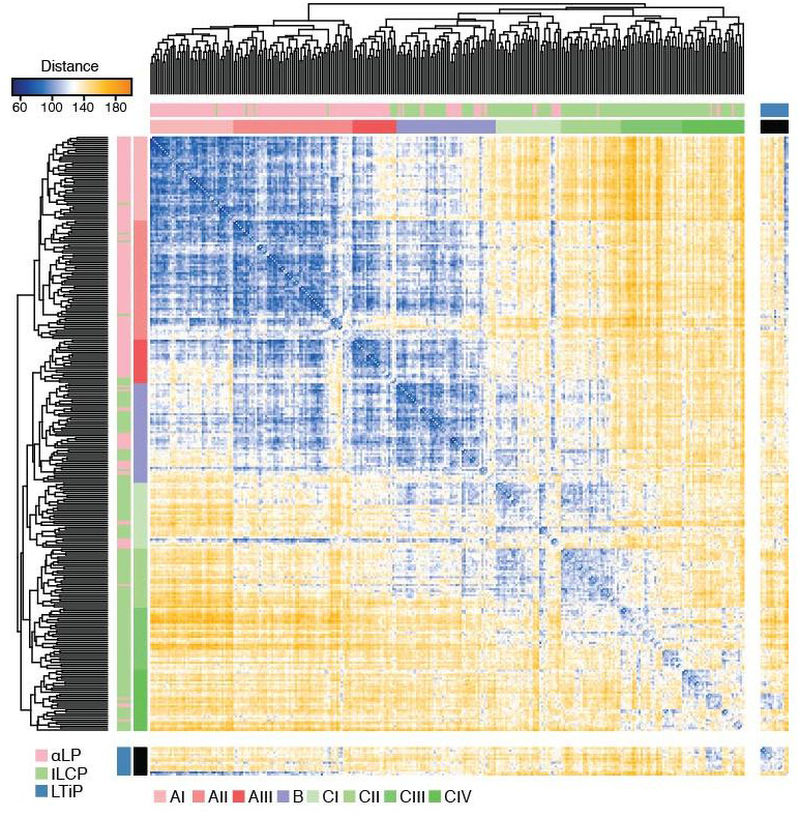
\includegraphics[width=0.8\textwidth]{figures/chapter3/S1}
\end{center}
	\caption{Intercellular transcriptional distances confirm hierarchical clustering analysis.} 
	Euclidean distance between all pairs of measured transcriptional profiles. Dendrograms shown are those obtained from the hierarchical clustering of these intercellular distances. Outer bar, sorted cell type; \aLP (red), ILCP (green), LTiP (blue). Inner bar, cluster assignment of each cell; AI--III (red), B (purple), CI--IV (green).
	\label{fig:chap3_S1}
\end{figure}

%% Chapter 3 Figure S2 mast cell %%
\begin{figure}[p]
\begin{center}
	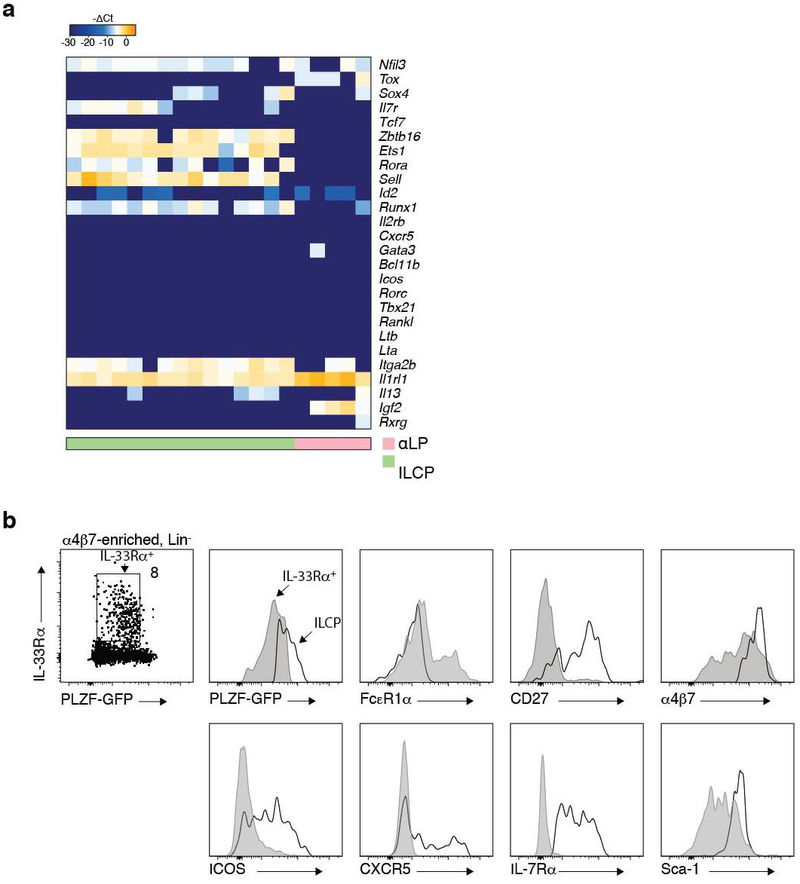
\includegraphics[width=0.8\textwidth]{figures/chapter3/S2}
\end{center}
	\caption{\ab\UP IL-33R$\alpha$\U{hi} cells represent contaminating mast cell precursors.} 
	a, Biomark analysis of the \textit{Il33r}\UP cluster excluded from the study suggested that they were not innate lymphoid cells, as evidenced by the nearly uniform lack of \textit{Tcf7} and \textit{Tox}, as well as other key markers. b, FACS analysis suggested the mast cell nature of these cells. \ab-MACS-enriched fetal liver cells obtained from the \textit{Zbtb16}-GFPCre reporter strain were gated as Lin\UM cells (this is the same population that was used to sort single \aLP and ILCP) and stained for IL-33R$\alpha$. The IL-33R$\alpha$\UP cells expressed intermediate amounts of PLZF (GFP) and \ab, possibly explaining why they were found as contaminants in the Biomark analysis of ‘purified’ \aLP and ILCP. 16\% of these cells expressed the mast cell marker Fc$\varepsilon$RI$\alpha$, indicating that they were mast cell lineage precursors.
	\label{fig:chap3_S2}
\end{figure}

%% Chapter 3 Figure S3 developmental progression %%
\begin{figure}[p]
\begin{center}
	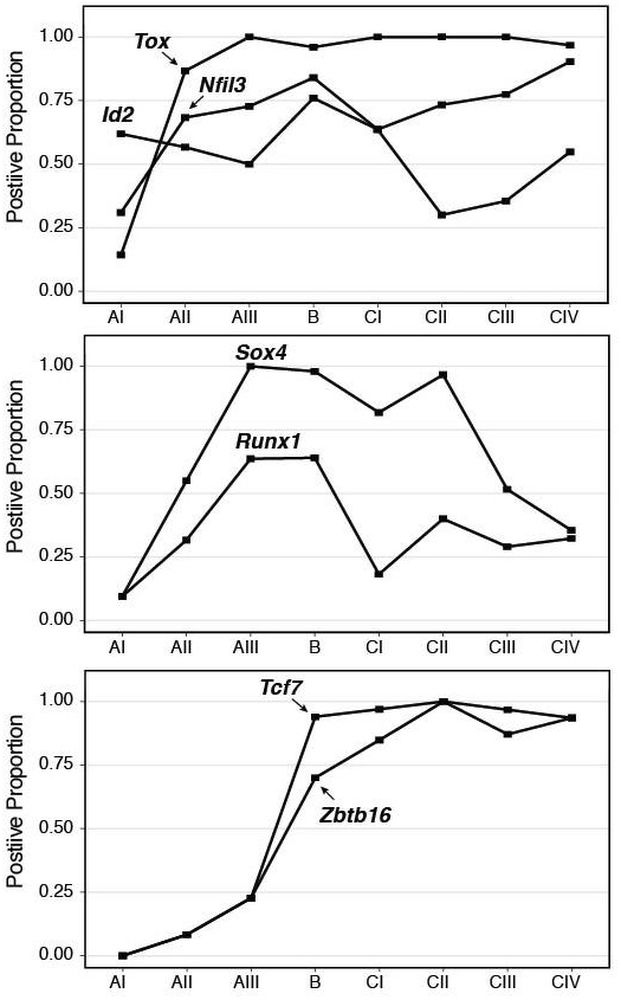
\includegraphics[width=0.6\textwidth]{figures/chapter3/S3}
\end{center}
	\caption{Expression frequencies of key transcription factors in \aLP and ILCP transcription-state clusters define their developmental progression.} 
	In each cluster, the proportion of cells with detectable levels of transcript is calculated for genes defining early developmental transitions. Similar to the trends observed in average transcript levels by cluster, \textit{Id2} is first expressed at a low level in AI, followed by \textit{Tox} and \textit{Nfil3} in AII, \textit{Sox4} and \textit{Runx1} in AIII, and finally by \textit{Tcf7} and \textit{Zbtb16} in B.
	\label{fig:chap3_S3}
\end{figure}


%% REVERT FIGURE NUMBERING %%
\renewcommand\thefigure{\thechapter.\arabic{figure}} 



%%% END CHAPTER 3 SINGLECELL %%%

